\section{Robust Structure From Motion}
\label{sec:sfm}

Given our Gaussian mixture model, we can now detect the similarity between
traces and use this probability to remove traces that decrease the quality of
performing structure from motion.  We first describe the application of our GMM
model to this problem, and then describe the setup and results of our
experiments.

\subsection{Model Application} % (fold)
\label{sub:Model Application}

In structure from motion, we focused on recovering the structure of a
static scene from a (possibly noisy) mobile camera.  We used our mobile phones,
an iPhone and Android, to collect data and found that unlike much original
research in the field, using an mobile phone by hand to capture video resulted
in highly unstable, shaky video.  The structure from motion algorithm works
fine with shaky video, but we found that SIFT and KLT often, as a result of
shaky, low-quality video, incorrectly traced features resulting in bad traces
and worsening the results for structure from motion.  Additionally, we found
that if there was a moving object in the video frame, it made it difficult for
the structure from motion algorithm to disentangle the motion of the object in
the scene from the motion of the camera, again worsening the results of the
structure from motion algorithm.  Sighting these two issues, we aimed to use or
GMM to improve the results of the structure from motion algorithm.

As explained previously, our GMM detects how similar traces are within a given
scene.  As a result, ``bad traces'' from incorrectly tracing a feature are
considered low probability traces since they are shaped quite differently from
correct traces matching the motion of the camera.  Similarly, moving objects in
a scene create create traces very different than those from static objects,
thus also giving them a low probability in our GMM.  When plotting a
distribution of these traces, as seen in Figure \ref{fig:logpdfs}, we see that
a relatively small percentage of the traces have a much lower probability than
a majority of the traces, which are of similar probability.  We consider this
segment of much lower probability traces to be outliers and thus should be
removed before performing the structure from motion algorithm.

\begin{figure}[h]
	\begin{subfigure}[b]{0.5\textwidth}
		\centering
		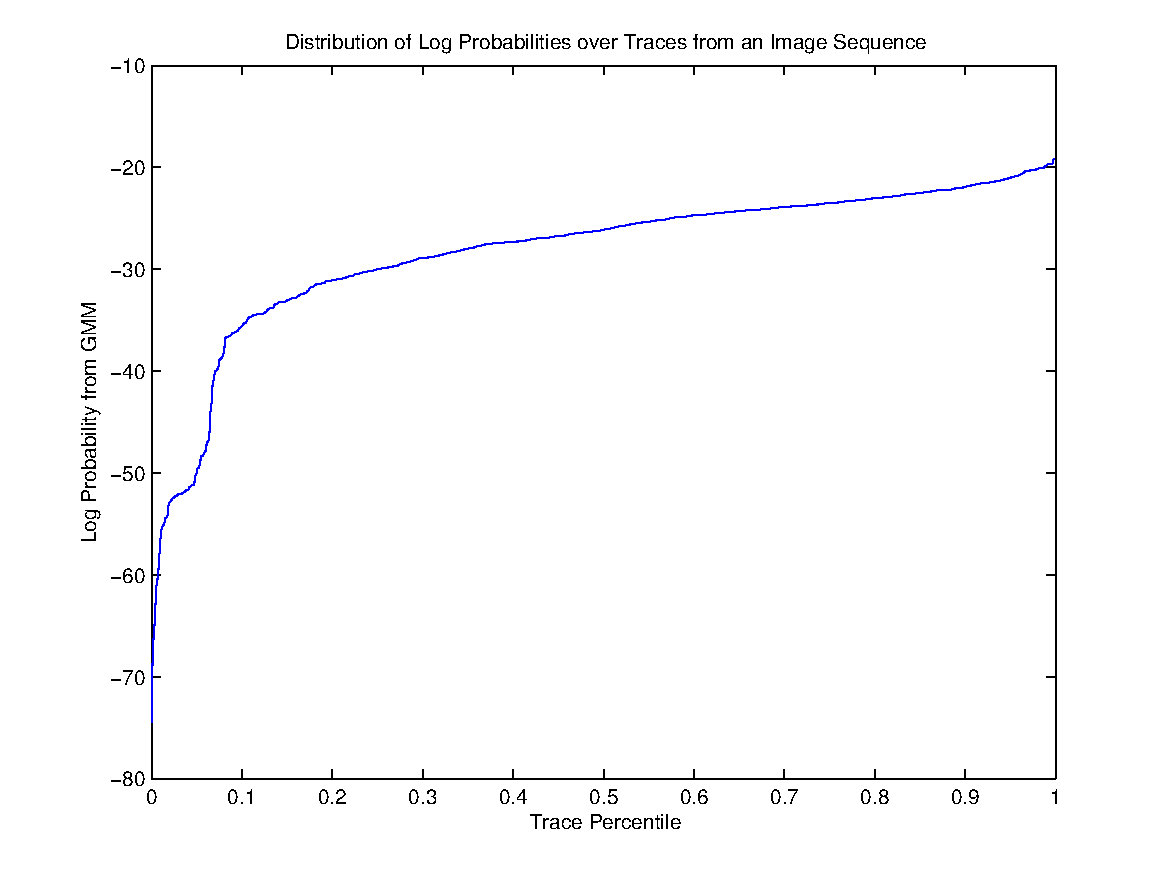
\includegraphics[width=0.9\textwidth]{figs/logpdfs-frame90.pdf}
		\caption{Outdoor dataset}
		\label{fig:logpdfs:90}
	\end{subfigure}%
	\begin{subfigure}[b]{0.5\textwidth}
		\centering
		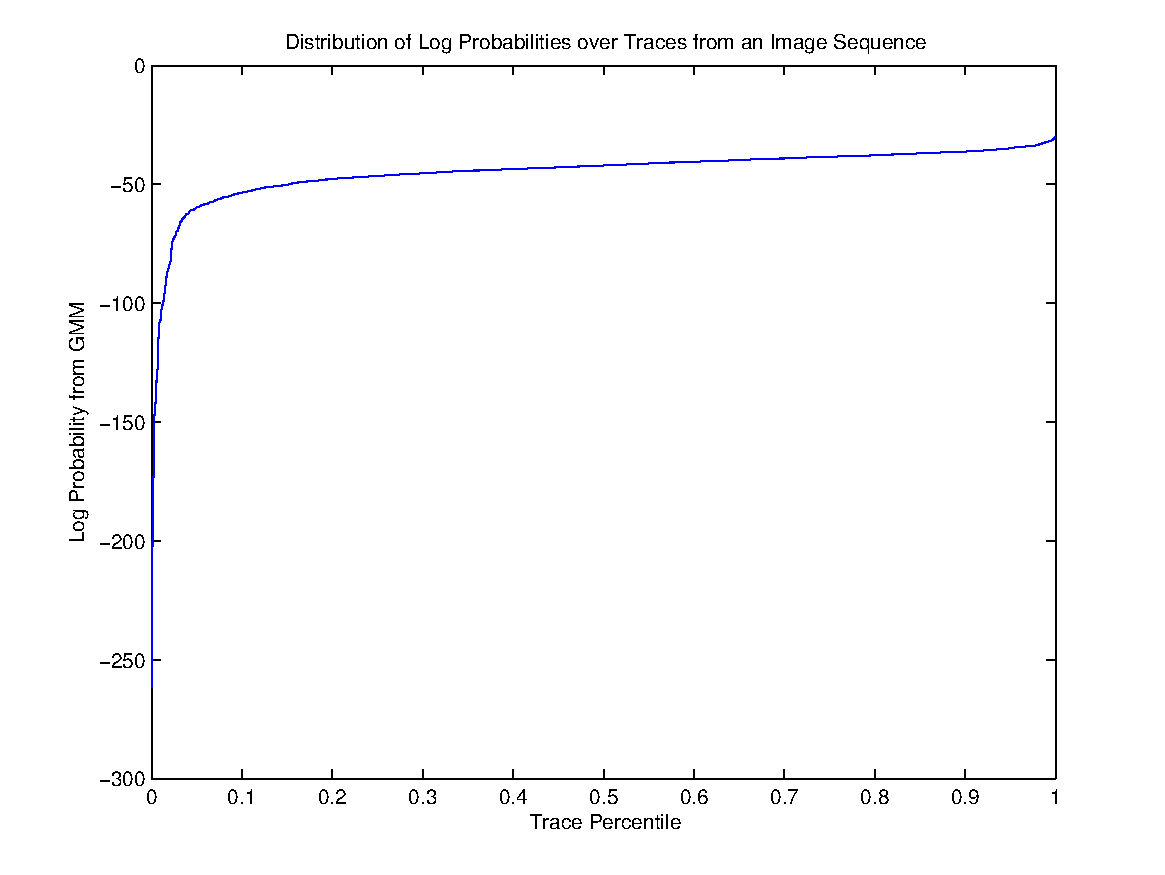
\includegraphics[width=0.9\textwidth]{figs/logpdfs.pdf}
		\caption{Outdoor dataset 2}
		\label{fig:logpdfs:105}
	\end{subfigure}%

	%\begin{center}
		%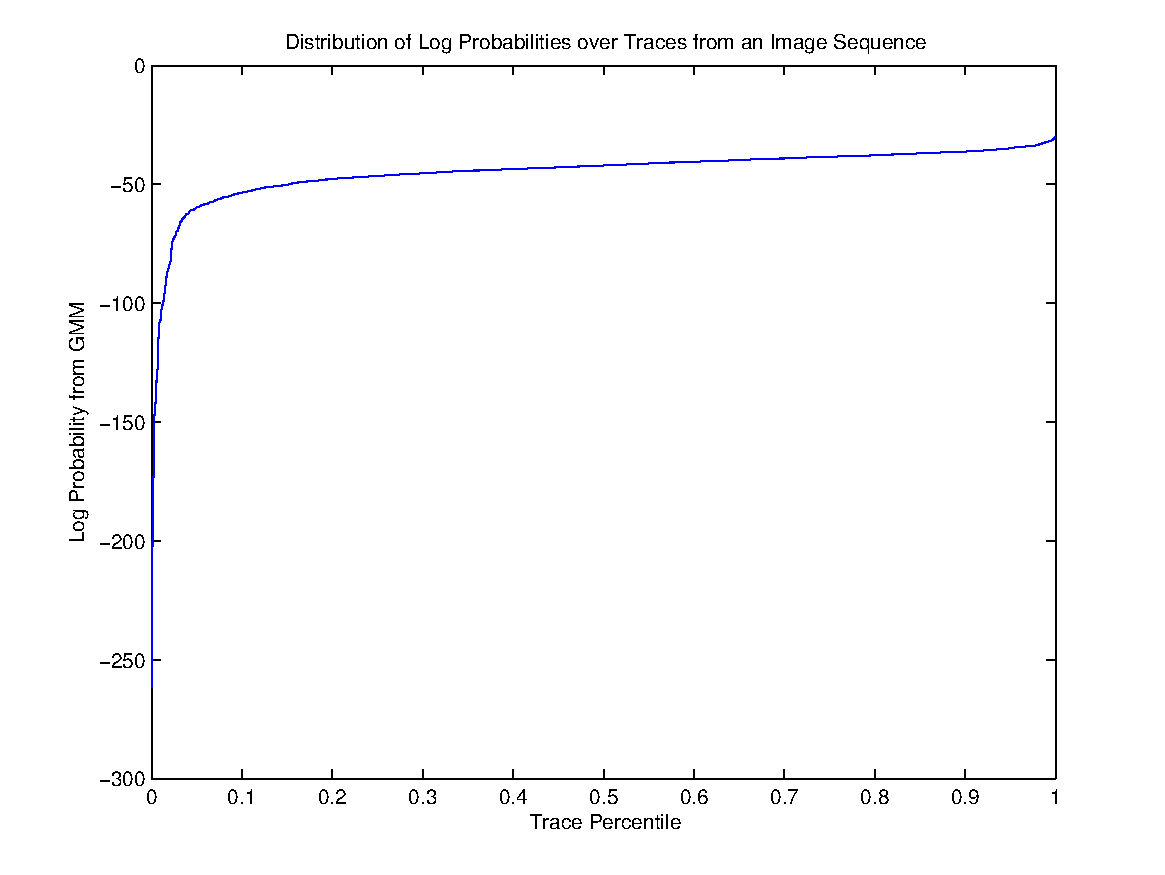
\includegraphics[width=4in]{figs/logpdfs.pdf}
	%\end{center}
	\caption{Distribution of log-probabilities generated by GMM for a set of traces in our ``Outdoor'' datasets}
	\label{fig:logpdfs}
\end{figure}

In our tests we found that approximately 10\% of traces were outliers, and thus
for simplicity using a simple thresholding mechanism, keeping only the top 90\%
of traces (based on their GMM score).  It is clear from the log probability
distributions from many videos, that our GMM generally produces distributions
similar to that in Figure \ref{fig:logpdfs}.  In future work, a more robust
method could be used to detect the change in log probability over trace
percentile and thus automatically find at what percentile is the ``best''
threshold.

% subsection Model Application (end)

\subsection{Experiments} % (fold)
\label{sub:Experiments}

\paragraph{Setup} 
To test our algorithm ran it on subsets of frames from multiple different data
sets: a desk chair, a lounge chair, and an outdoors scene.  For each we took a
subset of frames from the video so that a large number of points were tracked
across all frames, before running our algorithm.  For the desk chair we used 30
frames that tracked 164 features, for the lounge chair we used 20 frames that
tracked 508 features, and for the outdoor scene we used 10 frames that tracked
784 features and later in the video 15 frames that tracked 1596 features (which
we will refer to as ``Outdoors 2'').  In each video we have a substantial
amount of camera motion around a generally static scene.

\alex{nico - please expand on rank 3 thing here and check the rest of the description:}\\
To evaluate the effectiveness of the structure from motion algorithm we compare
a ratio of singular values from the singular value decomposition.  In each case
we take the SVD of the $W$ matrix and analyze the singular values in the
resulting $\Sigma$ matrix, where $\sigma_i$ is the $i$-th singular value.
Because the scene is three dimensional, we expect the data to be rank three,
and therefore ideally $\sigma_i$ for $1 \leq i \leq 3$ to be large and $\sigma_i$ for $i
> 3$ to be very small.  We therefore denote the following ratio as the purity
score for a given $W$ as computed by the SVD:
\begin{align}
	{\rm Purity\ Score} &= \frac{\sigma_1}{\sum_{i > 3} \sigma_i}.
\end{align}
Because all $\sigma_i$ in the denominator should be small, the larger the
purity score, the more clean the data in $W$ is and the better the result of
structure from motion.

\paragraph{Results} 

To visually evaluate the effectiveness of our methodology, we looked at the
distribution of log-probabilities as was discussed previously in Figure
\ref{fig:logpdfs}, as well as overlaying the trace scores on a frame from the
video, as can be seen in Figure \ref{fig:colored-traces}.  In these figures, we
color traces across a spectrum based on each trace's GMM score.  Traces with
higher probability are colored green, and traces with lower probability are
colored red. 

In Figure \ref{fig:colored-traces}(a) and (b) we see that feature tracking
algorithm occasionally finds faulty traces when trying to track a feature along
the carpet.  In each case we see that the shape of the trace is largely
different than that of other traces in the scene.  In Figure
\ref{fig:colored-traces}(c), the algorithm notices that a man walked through
the middle of the scene while filming it.  As a result, his traces show his
motion as well as the camera motion and are largely different than the traces
from the static objects in the scene.  Our algorithm successfully detects this
and gives these traces a low probability through the GMM.

\begin{figure}[tb]
	\hspace{-0.6cm}
	\begin{minipage}[b]{0.5\linewidth}
		\centering
		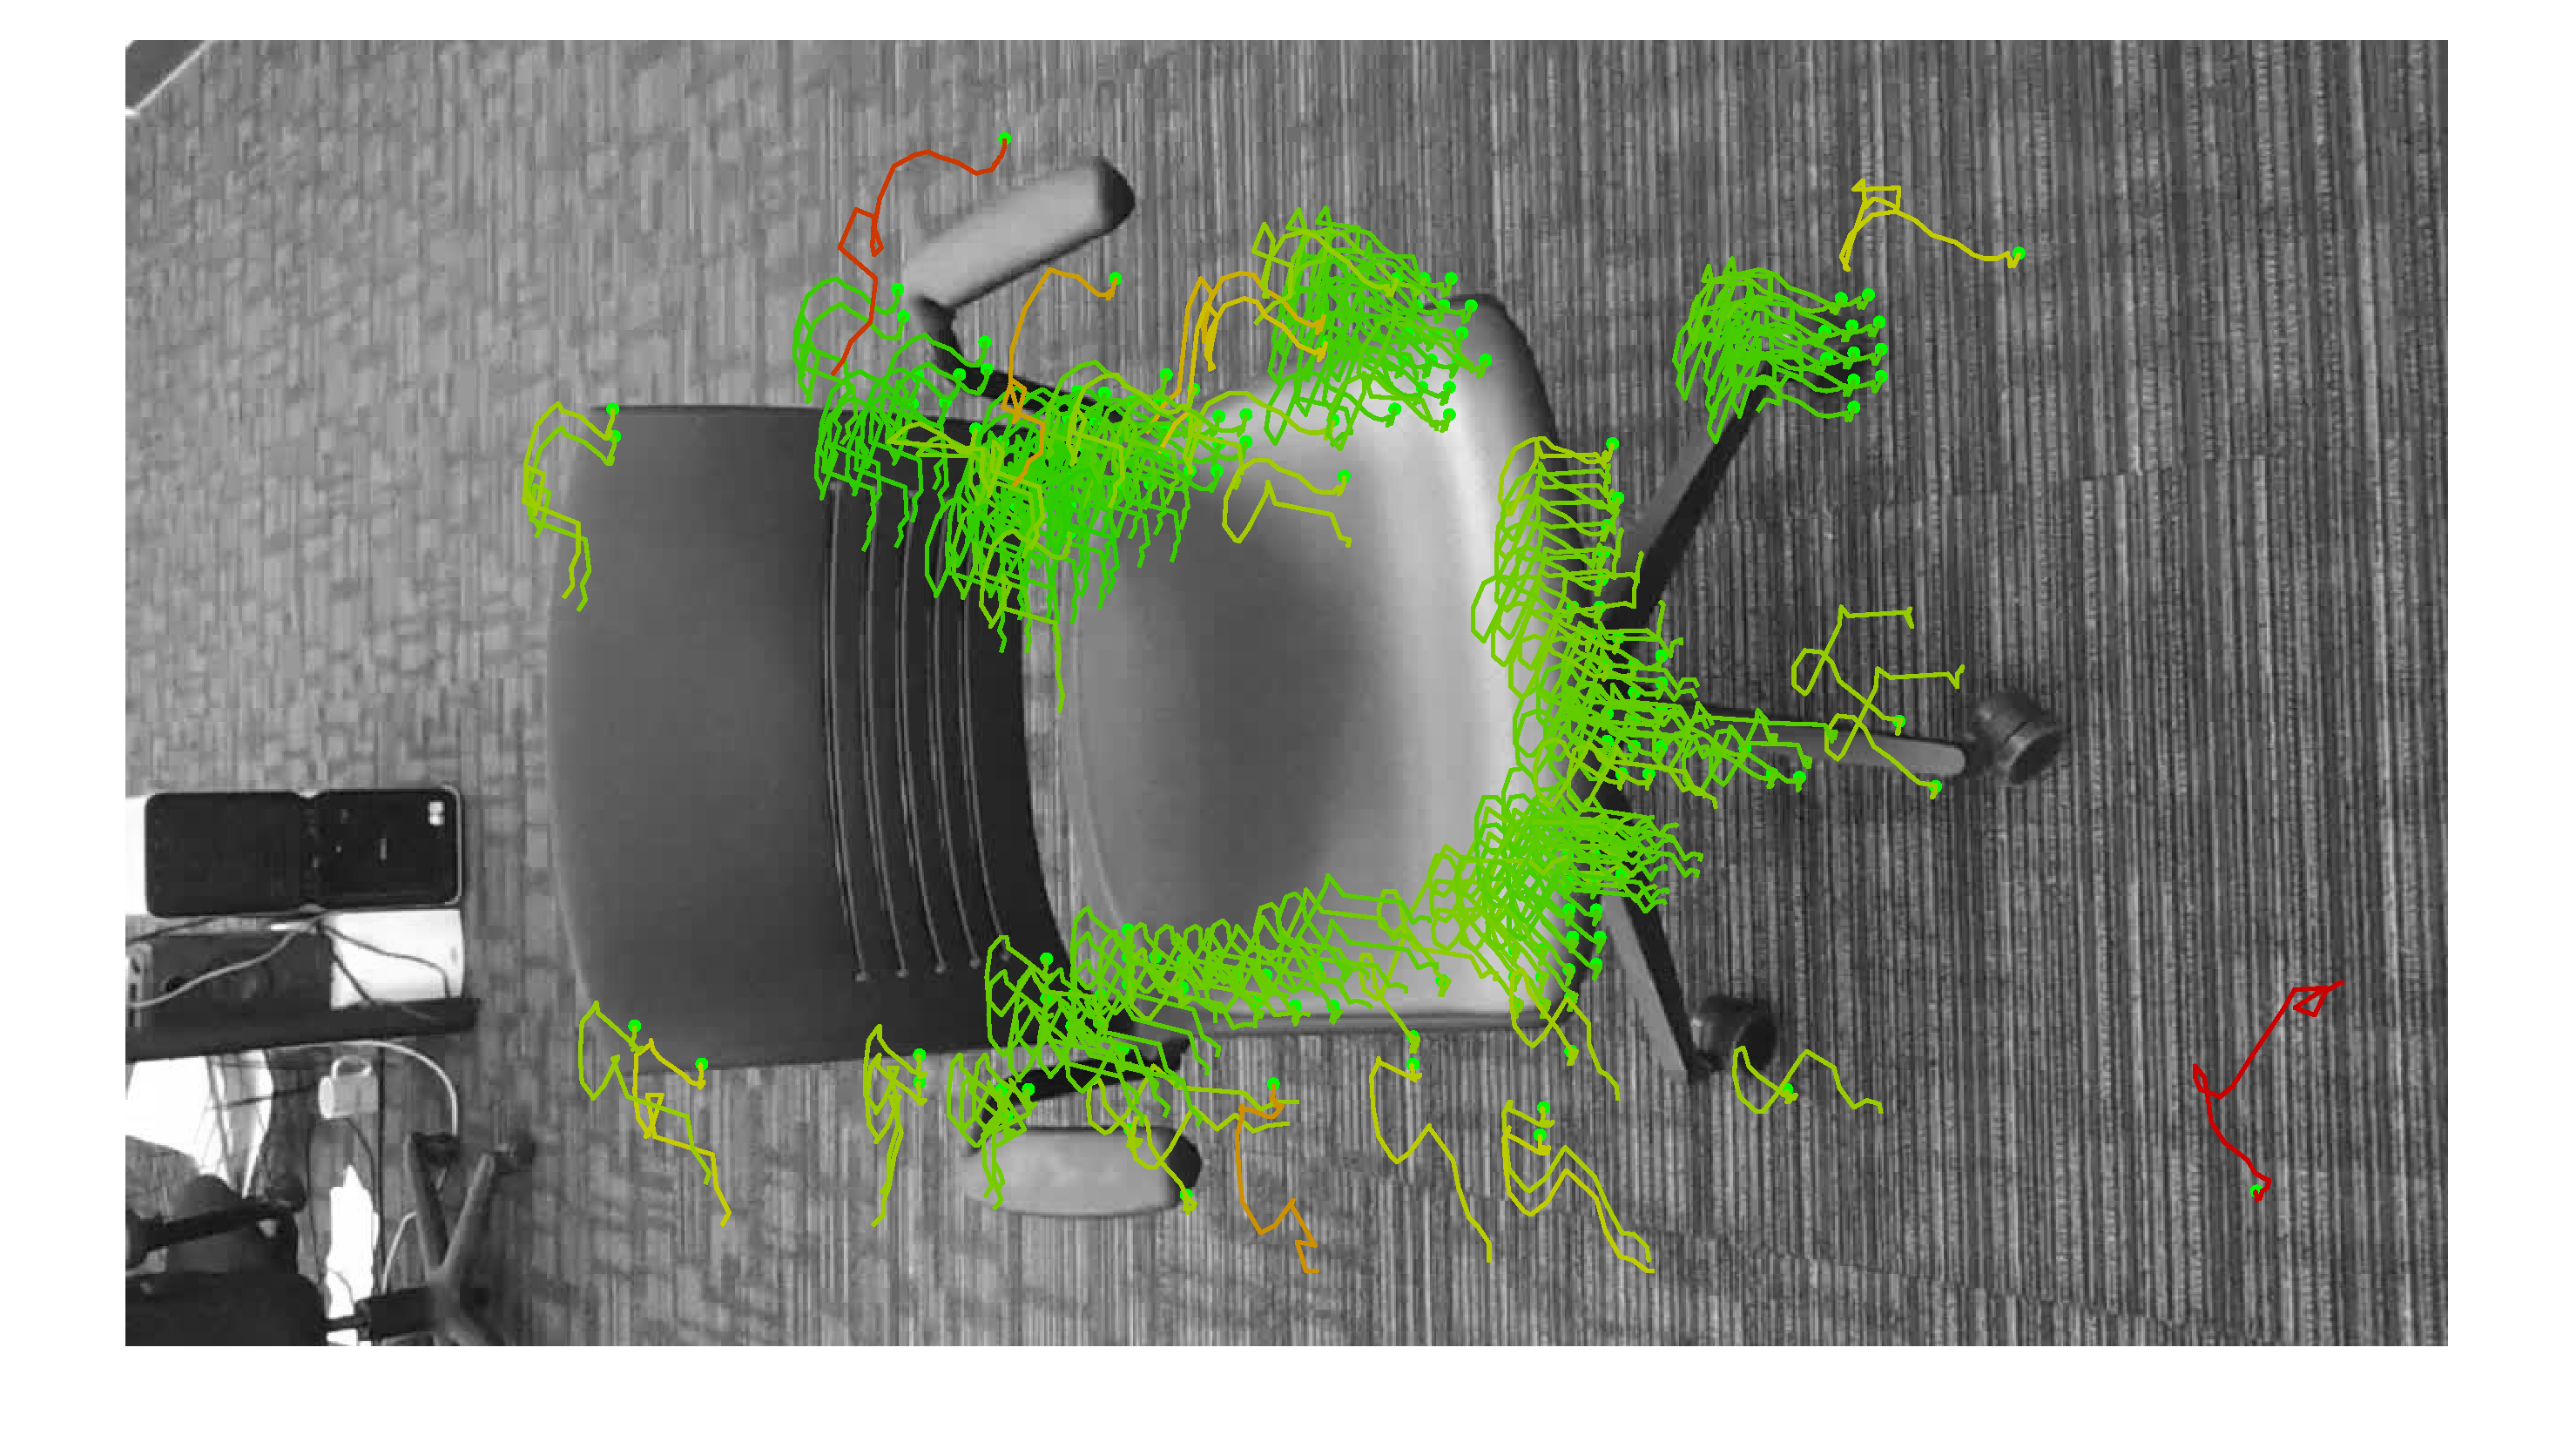
\includegraphics[height=2.1in,angle=-90]{figs/desk-1.pdf}\\ (a)
		%\caption{default}
	\end{minipage}
	\hspace{0cm}
	\begin{minipage}[b]{0.5\linewidth}
		\centering
		\begin{minipage}[b]{\linewidth}
			\centering
			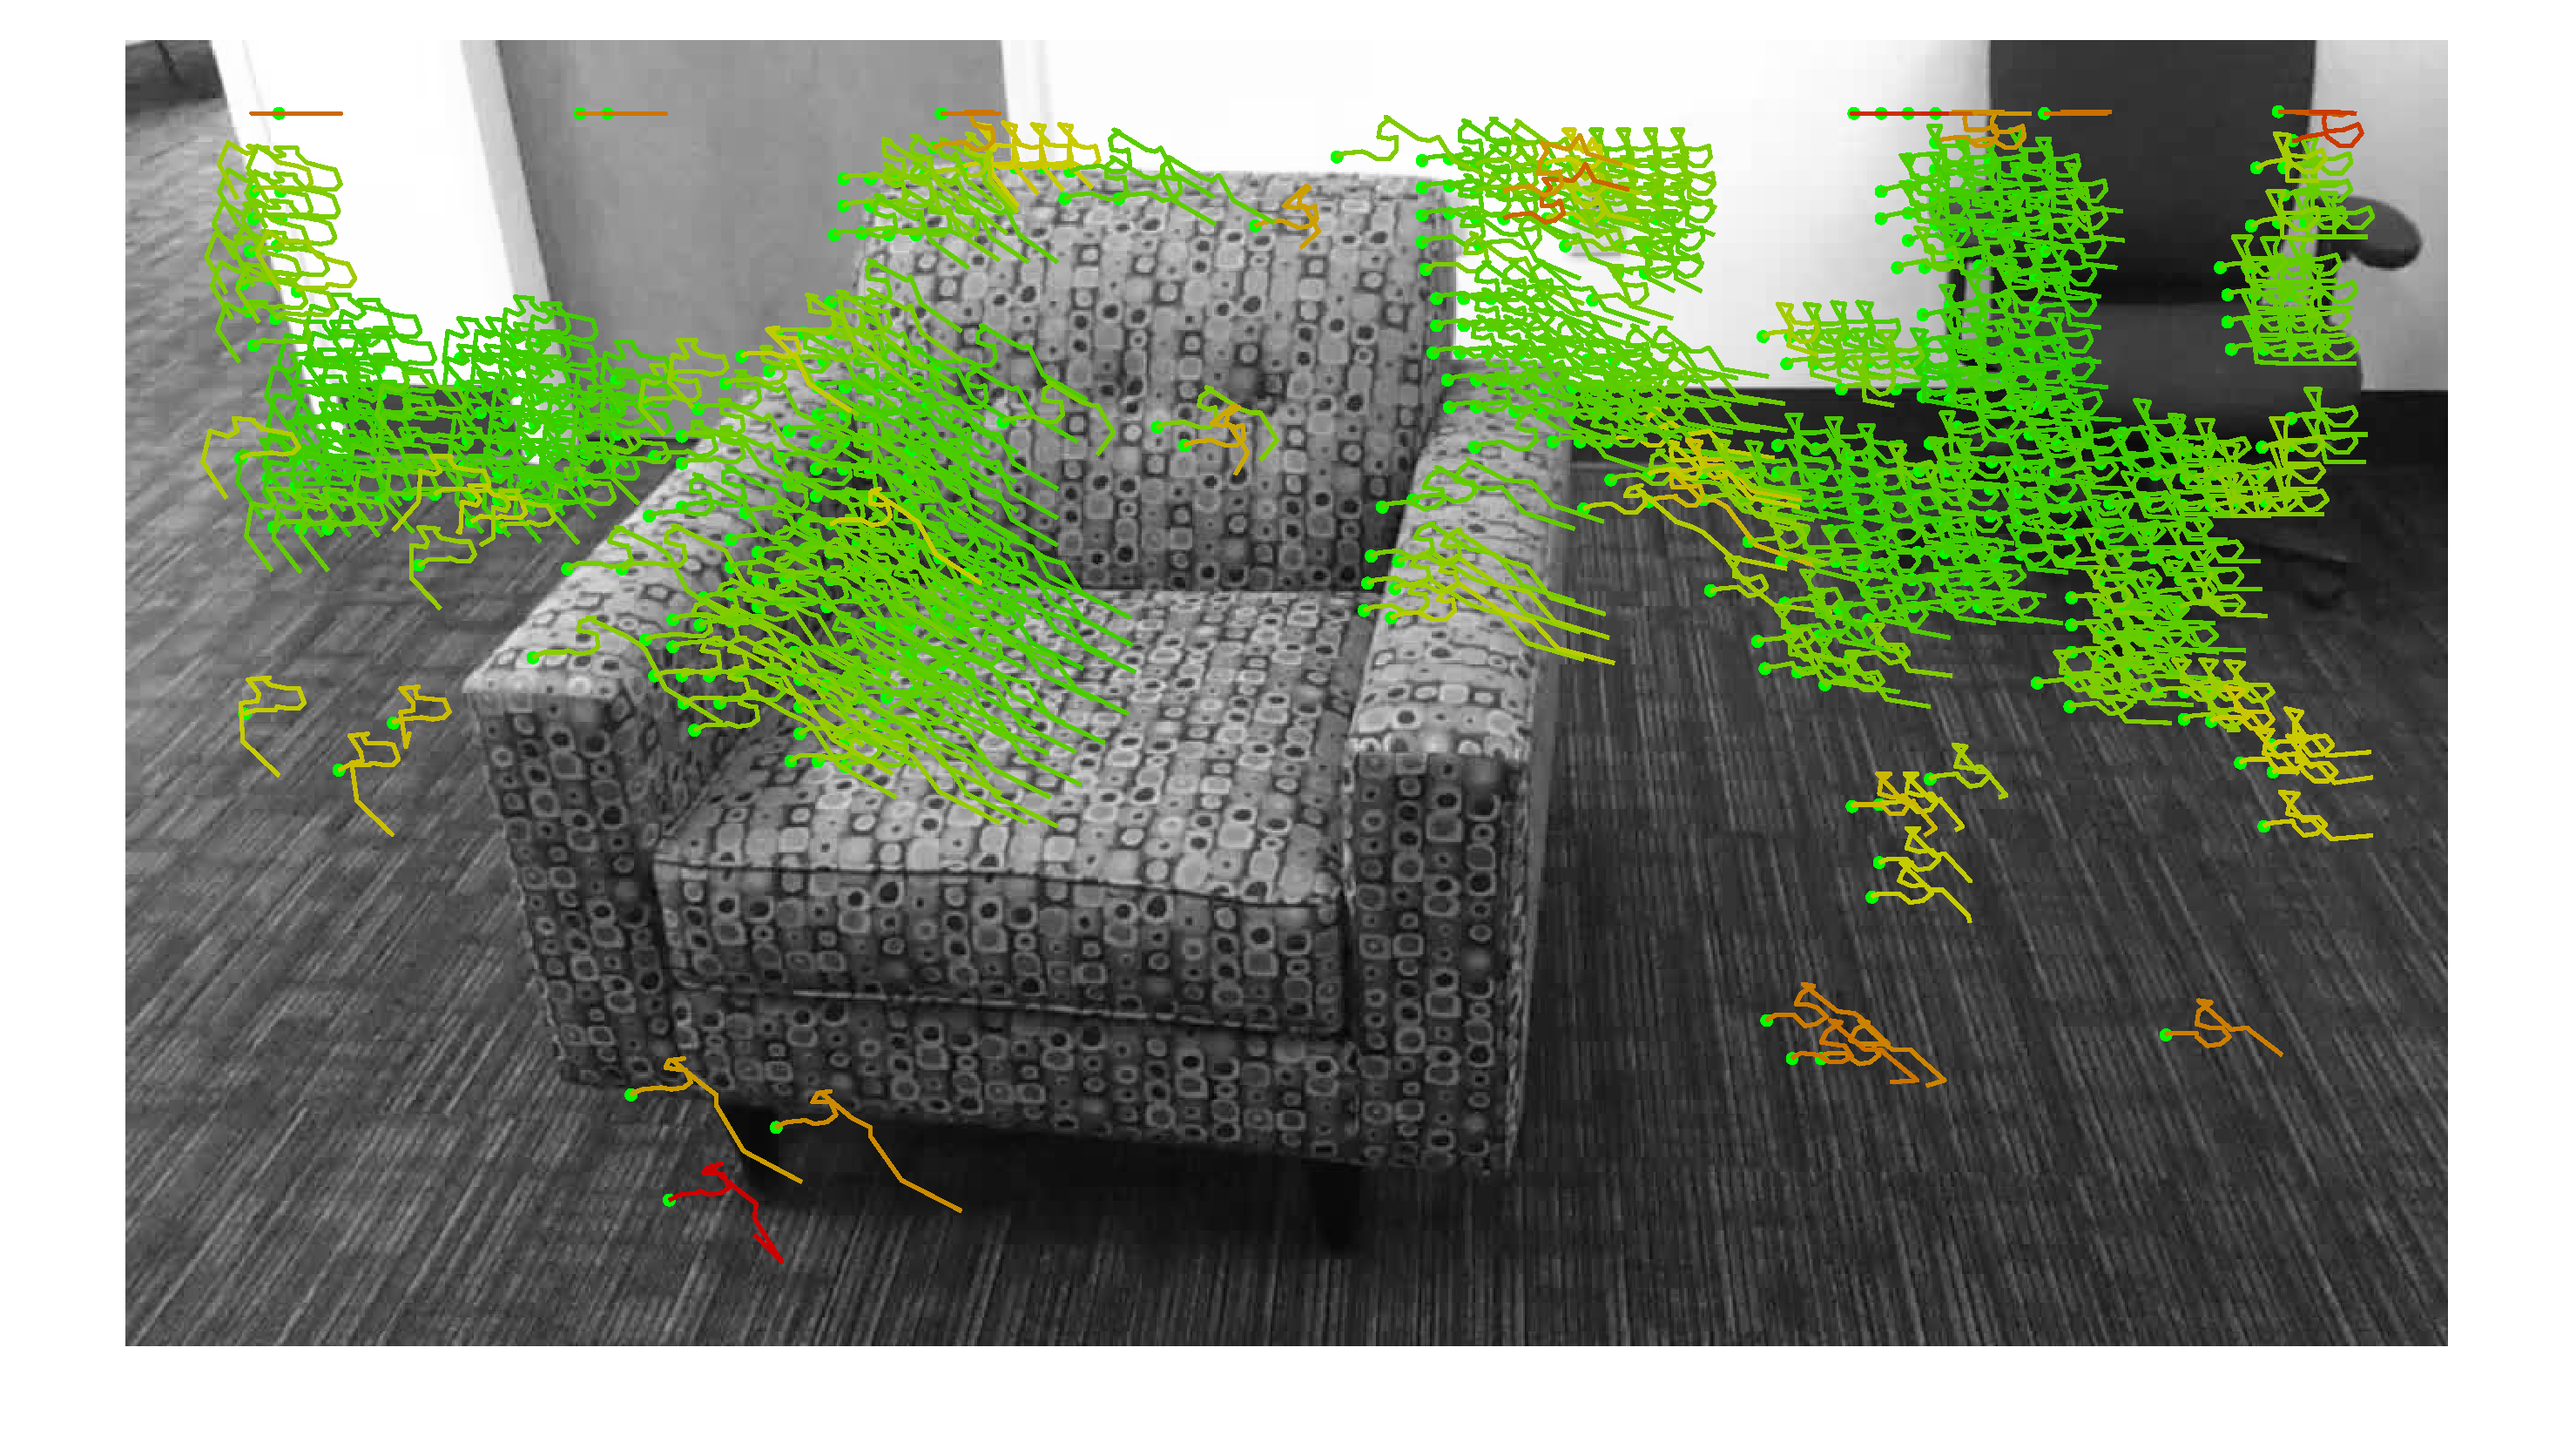
\includegraphics[width=3in]{figs/lounge-1.pdf} \\ (b)
			%\caption{default}
		\end{minipage}
		\vspace{0.1cm}
		\begin{minipage}[b]{\linewidth}
			\centering
			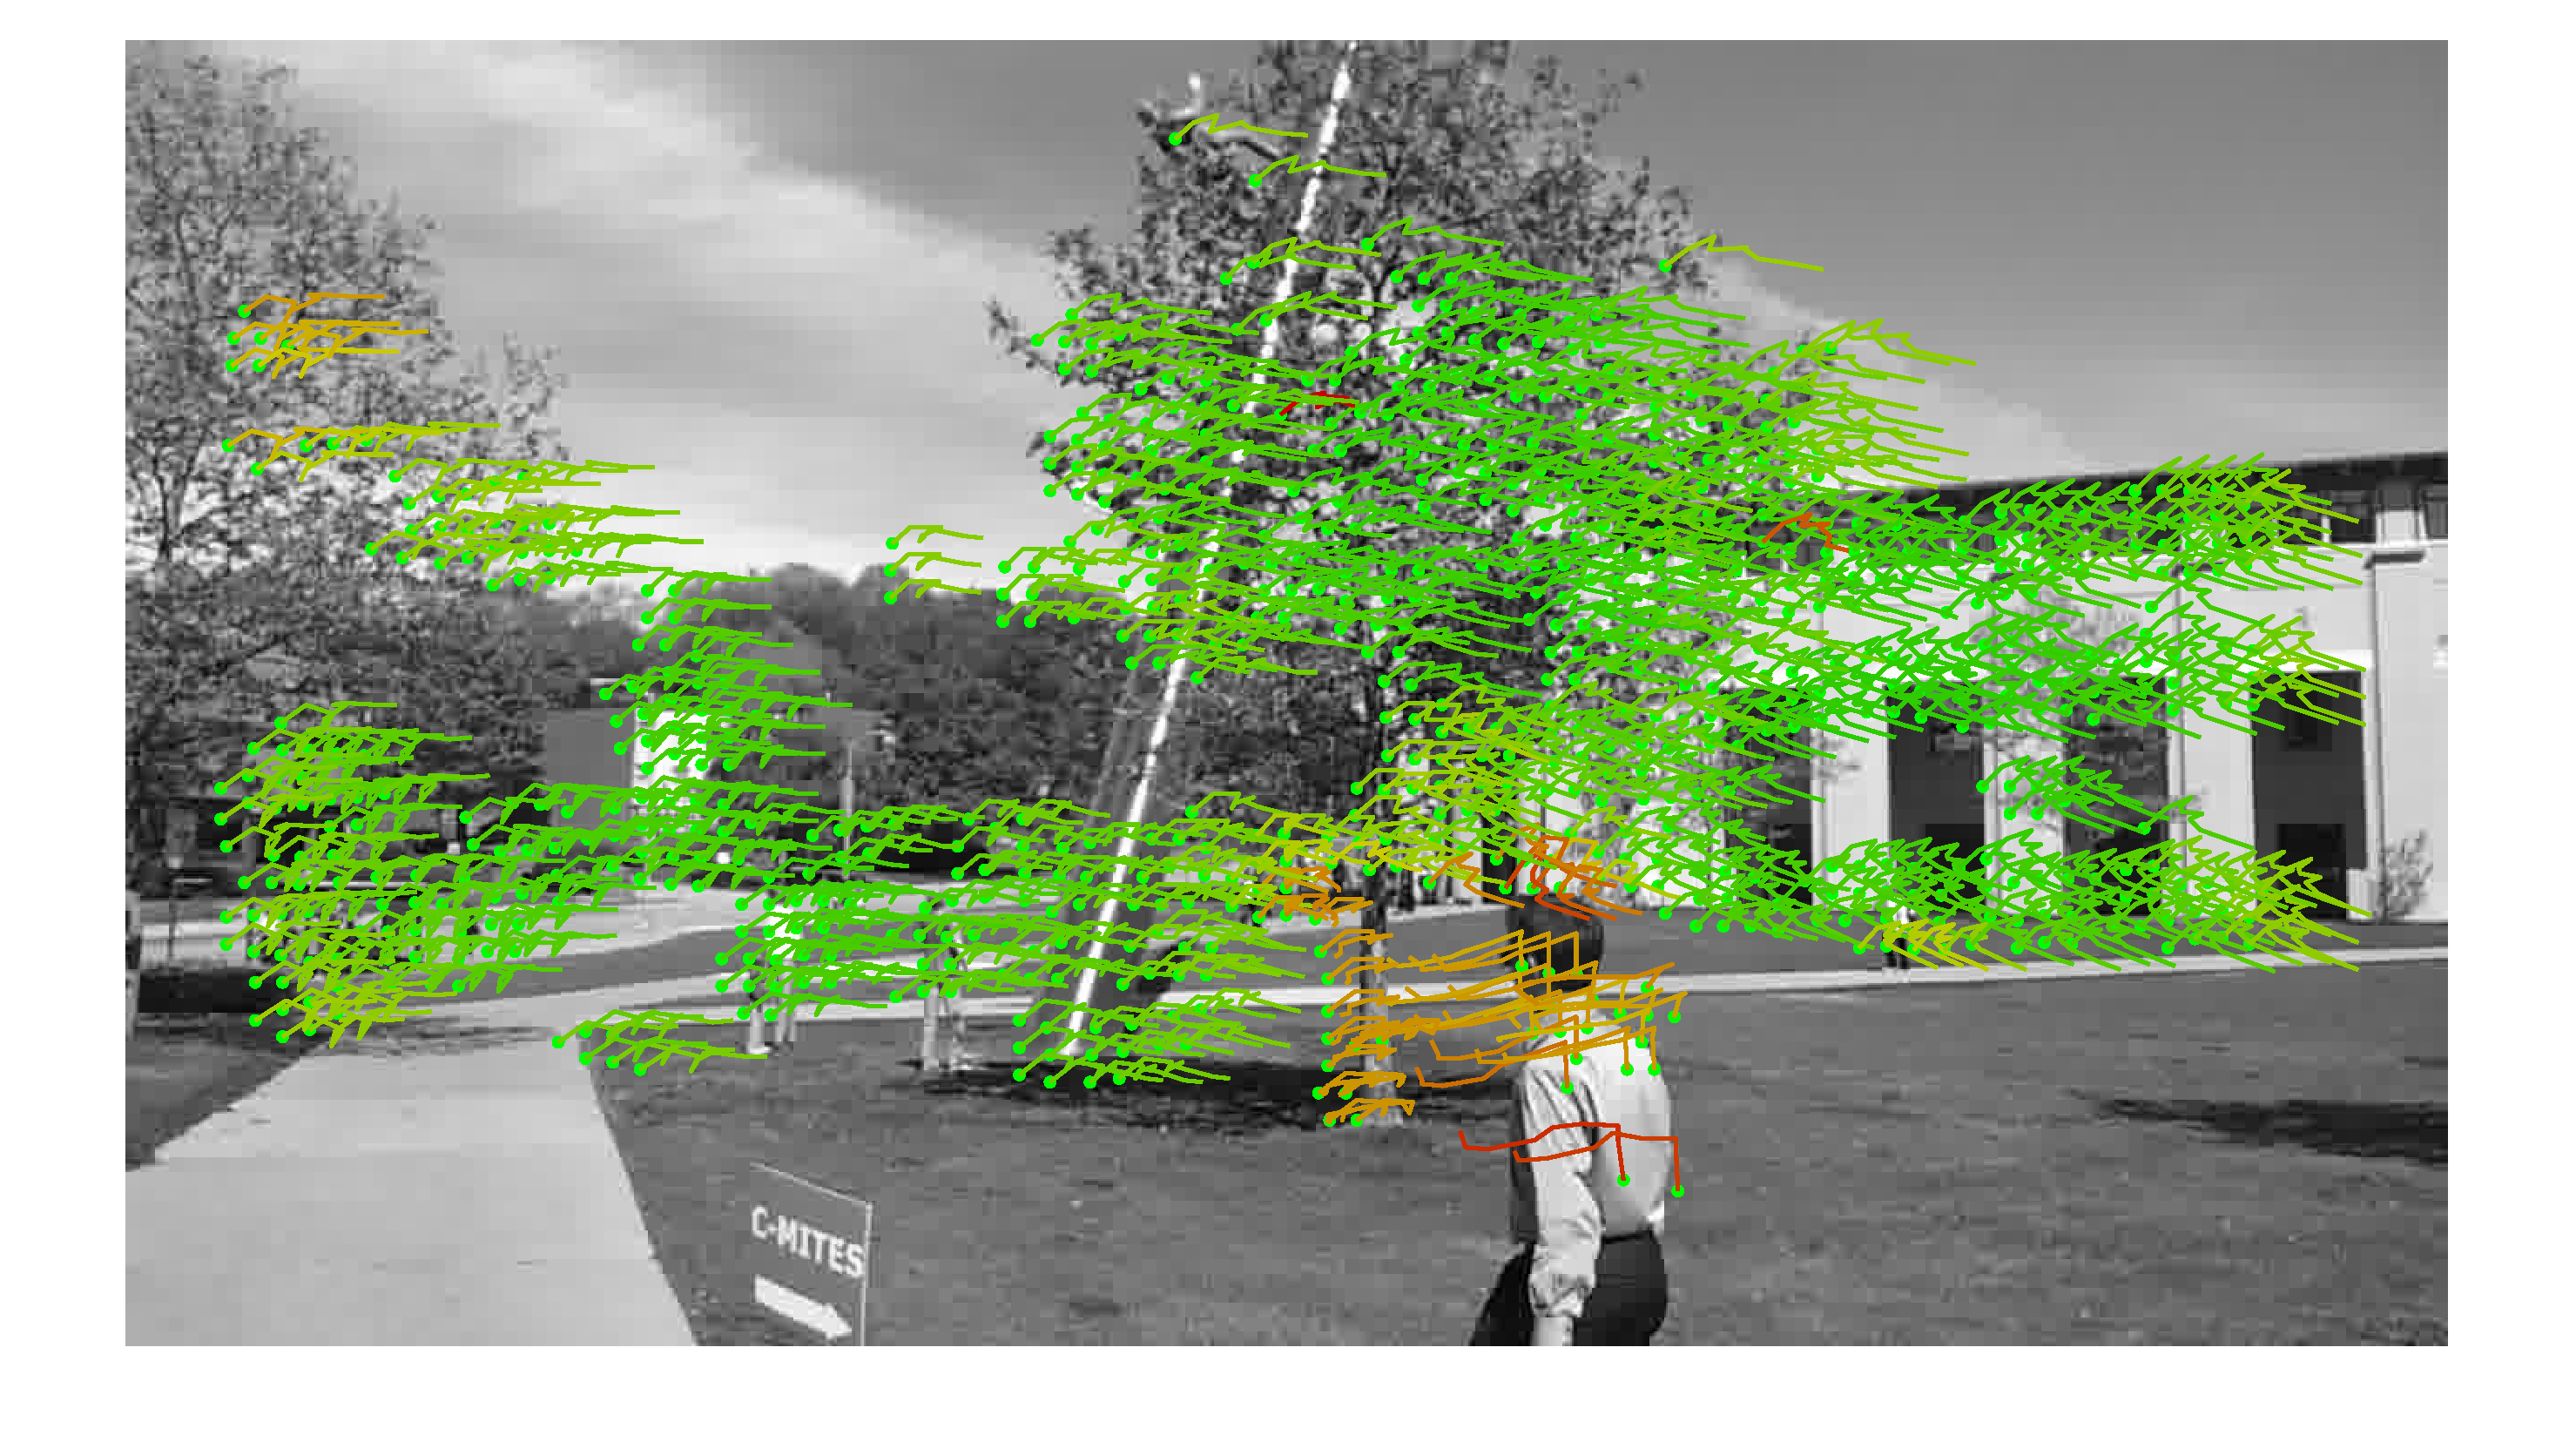
\includegraphics[width=3in]{figs/outdoor3-90.pdf} \\ (c)
			%\caption{default}
		\end{minipage}

	\end{minipage}
	\caption{Traces colored by GMM score for (a) desk chair, (b) lounge chair, and (c) outdoors.  Green reflects a high GMM score and red reflects a low GMM score.}
	\label{fig:colored-traces}
\end{figure}


In addition to visually evaluating the success of our algorithm in isolating
outlier traces, we compared the purity score of the data before and after
outlier removal.  In running our algorithm and evaluation across all four data
sets, we found that in every case outlier removal improved the purity score and
thus structure from motion result.  The purity score comparison can be seen in
Table \ref{tab:purities}.  Not surprisingly, the algorithm seems to be most
useful when there is a moving object in the scene, as this results in a large
number of outlier points that would disrupt the structure from motion
algorithm.  Overall, we considered our method to work as intended and improved
the resulting structure from motion.

\begin{table}[tb]
	\begin{center}
		\begin{tabular}{|l|c|c|}
			\hline
			\multirow{2}{*}{Data Set}  &\multicolumn{2}{|c|}{Purity Score}\\ \cline{2-3}
			& \multicolumn{1}{|c|}{Original}  & \multicolumn{1}{|c|}{With Outlier Removal}\\ \hline
			Desk Chair & 36.14 & 40.63 \\ \hline
			Lounge Chair & 89.2 & 111.36 \\ \hline
			Outdoors & 90.43 & 175.44 \\ \hline
			Outdoors 2 & 96.37 & 127.96 \\ \hline
		\end{tabular}
	\end{center}
	\caption{Comparison of Purity Score before and after outlier removal.}
	\label{tab:purities}
\end{table}


% subsection Experiments (end)
